\documentclass{jarticle}
\usepackage{amsmath,amssymb}
\usepackage{amsmath}
\usepackage[dvipdfmx]{graphicx}
\usepackage{here}
\usepackage{pifont}
\usepackage[left=2cm, right=2cm]{geometry}
\setcounter{MaxMatrixCols}{20}
\begin{document}
\section{結果(2)}
先と同様に$\mathcal{H}$を数値計算で対角化していく。
$N=1000$、$k_y$を横軸として変化させて縦軸に固有値をプロットし分散関係を描いた。結果は以下のようになった。\\
\begin{figure}[H]
	\centering
	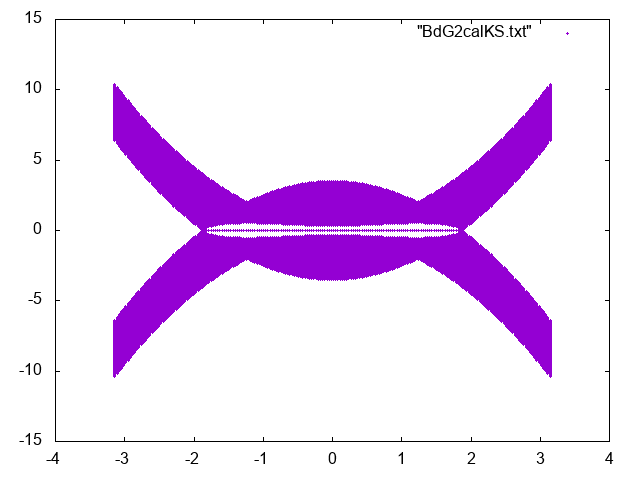
\includegraphics[scale=0.7]{BdG2calKS.png}
	\caption{分散関係}
\end{figure}
次にグリーン関数を用いて状態密度を求めた。
端には電子が存在しており、その間にエネルギー状態があるが、周りにはないことが分かる。\\
次に$E$を$-3$〜$3$で動かして$\rho$をプロットした。この時$\delta=10^{-3}$とした。
以下に結果を示す。
\begin{figure}[H]
	\centering
	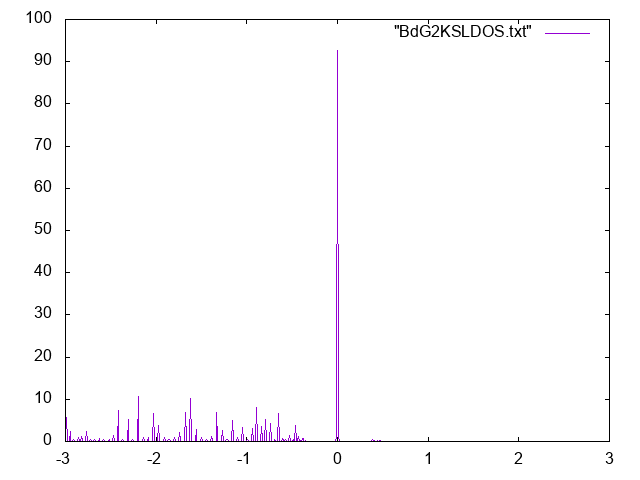
\includegraphics[scale=0.7]{BdGKSLDOSedge.png}
	\caption{表面の状態密度}
\end{figure}
ここからエネルギーが$-1$〜$1$では状態があることが分かる。これは(1)の結果とは異なる点である。\\
また内部を
\begin{align}
\rho=-\dfrac{1}{\pi}Im(G_{201,202}+G_{202,202})
\end{align}
で求めると
\begin{figure}[H]
	\centering
	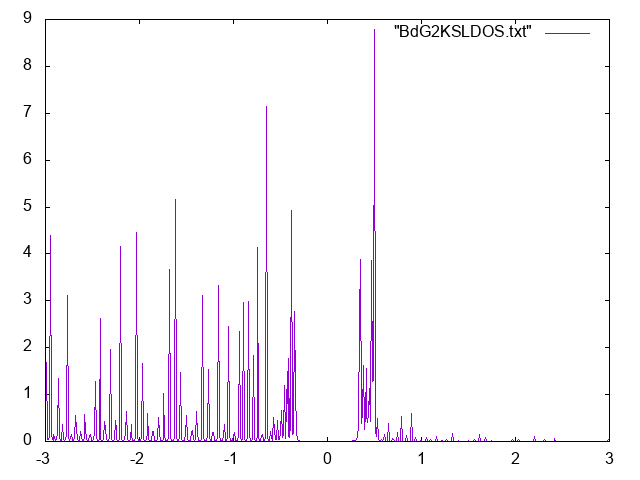
\includegraphics[scale=0.7]{BdGKSLDOSinternal.png}
	\caption{内部の状態密度}
\end{figure}
のようになり、$0$付近では(1)と同じように状態がない。
\end{document}